\newcommand{\graficotempo}{
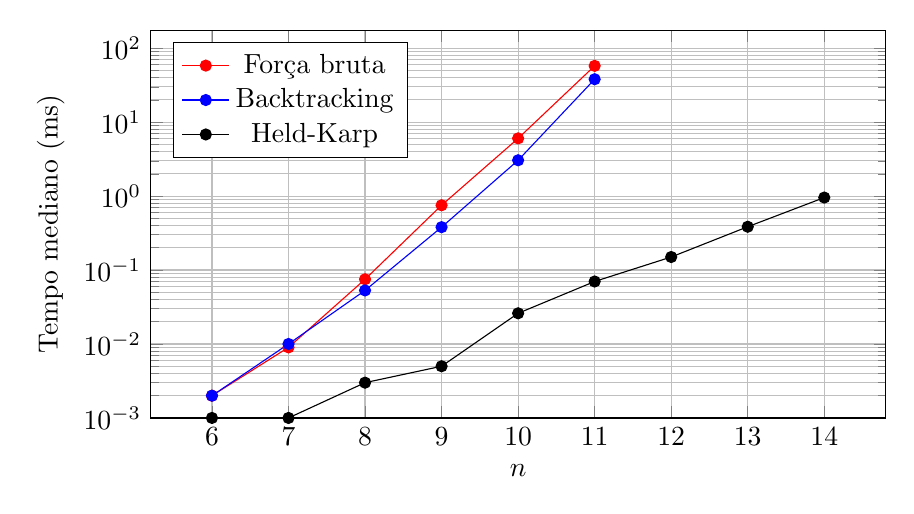
\begin{tikzpicture}\begin{semilogyaxis}[width=0.9\linewidth,height=6.5cm,xlabel={$n$},ylabel={Tempo mediano (ms)},legend pos=north west,grid=both,xtick={6,7,8,9,10,11,12,13,14},ymin=1e-3]
\addplot[color=red,mark=*] coordinates {(6,0.002) (7,0.009) (8,0.075) (9,0.751) (10,6.029) (11,57.604)};\addlegendentry{Força bruta}
\addplot[color=blue,mark=*] coordinates {(6,0.002) (7,0.010) (8,0.053) (9,0.380) (10,3.049) (11,38.012)};\addlegendentry{Backtracking}
\addplot[color=black,mark=*] coordinates {(6,0.001) (7,0.001) (8,0.003) (9,0.005) (10,0.026) (11,0.070) (12,0.150) (13,0.385) (14,0.955)};\addlegendentry{Held-Karp}
\end{semilogyaxis}\end{tikzpicture}}
\newcommand{\graficonos}{
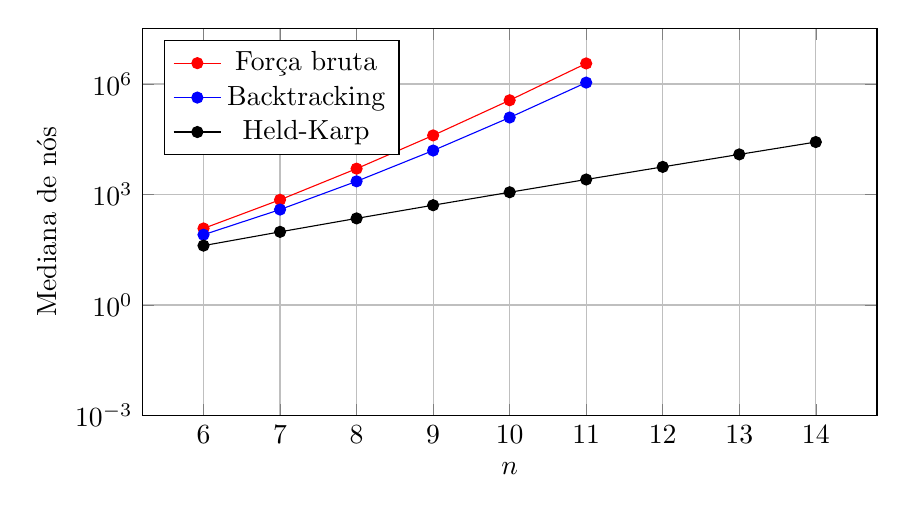
\begin{tikzpicture}\begin{semilogyaxis}[width=0.9\linewidth,height=6.5cm,xlabel={$n$},ylabel={Mediana de nós},legend pos=north west,grid=both,xtick={6,7,8,9,10,11,12,13,14},ymin=1e-3]
\addplot[color=red,mark=*] coordinates {(6,120.000) (7,720.000) (8,5040.000) (9,40320.000) (10,362880.000) (11,3628800.000)};\addlegendentry{Força bruta}
\addplot[color=blue,mark=*] coordinates {(6,81.000) (7,391.000) (8,2283.000) (9,15657.000) (10,123301.000) (11,1096011.000)};\addlegendentry{Backtracking}
\addplot[color=black,mark=*] coordinates {(6,41.000) (7,97.000) (8,225.000) (9,513.000) (10,1153.000) (11,2561.000) (12,5633.000) (13,12289.000) (14,26625.000)};\addlegendentry{Held-Karp}
\end{semilogyaxis}\end{tikzpicture}}
\newcommand{\tabelafiltro}{
\begin{tabular}{r rr}\toprule $n$ & nós com filtro & nós sem filtro\\ \midrule
6 & 0 & 6\\
7 & 0 & 16\\
8 & 0 & 14\\
9 & 0 & 15\\
10 & 0 & 44\\
11 & 0 & 31\\
\bottomrule\end{tabular}}
\newcommand{\tabelapiorcaso}{
\begin{tabular}{r rr rr rr}\toprule & \multicolumn{2}{c}{Força bruta} & \multicolumn{2}{c}{Backtracking} & \multicolumn{2}{c}{Held-Karp}\\ $n$ & nós & ms & nós & ms & nós & ms\\ \midrule
6 & 120 & 0.002 & 81 & 0.002 & 41 & 0.001\\
7 & 720 & 0.009 & 391 & 0.010 & 97 & 0.001\\
8 & 5040 & 0.075 & 2283 & 0.053 & 225 & 0.003\\
9 & 40320 & 0.751 & 15657 & 0.380 & 513 & 0.005\\
10 & 362880 & 6.029 & 123301 & 3.049 & 1153 & 0.026\\
11 & 3628800 & 57.604 & 1096011 & 38.012 & 2561 & 0.070\\
12 & -- & -- & -- & -- & 5633 & 0.150\\
13 & -- & -- & -- & -- & 12289 & 0.385\\
14 & -- & -- & -- & -- & 26625 & 0.955\\
\bottomrule\end{tabular}}
\newcommand{\tabelaheuristicas}{
\begin{tabular}{l r rrr}\toprule Tipo & Digrafos com ciclo & Guloso índice & Guloso Warnsdorff & Recozimento\\ \midrule
Ciclo + arcos extras & 72 & 48/48 & 10/48 & 47/48\\
DAG aleatório & 0 & -- & -- & --\\
Erdős–Rényi, $p=0{,}35$ & 41 & 1/27 & 0/27 & 27/27\\
Erdős–Rényi, $p=\ln n/n$ & 3 & 0/3 & 0/3 & 3/3\\
Torneio aleatório & 62 & 6/42 & 3/42 & 42/42\\
Pior caso (sem ciclo) & 0 & -- & -- & --\\
\bottomrule\end{tabular}}
\newcommand{\tabelatipos}{
\begin{tabular}{l rr rr rr}\toprule & \multicolumn{2}{c}{Força bruta} & \multicolumn{2}{c}{Backtracking (Warnsdorff)} & \multicolumn{2}{c}{Held-Karp}\\ Tipo ($n=11$) & mediana & máximo & mediana & máximo & mediana & máximo\\ \midrule
Ciclo + arcos extras & 0.000 & 0.000 & 0.001 & 0.002 & 0.004 & 0.049\\
DAG aleatório & 0.000 & 0.000 & 0.000 & 0.000 & 0.000 & 0.001\\
Erdős–Rényi, $p=0{,}35$ & 3.131 & 36.111 & 0.005 & 0.030 & 0.016 & 0.044\\
Erdős–Rényi, $p=\ln n/n$ & 0.000 & 0.000 & 0.000 & 0.000 & 0.001 & 0.001\\
Torneio aleatório & 0.822 & 14.243 & 0.002 & 0.039 & 0.058 & 0.076\\
\bottomrule\end{tabular}}
\newcommand{\totalmedicoes}{2528}\newcommand{\totalcensurados}{0}
